%Title: Fus. evap results for U and Th isotopes
%Author: A. Raggio
%Year: 2020

\documentclass[10pt]{beamer}

%
%Setting file
%

\usepackage[T1]{fontenc}
\usepackage[utf8]{inputenc}

\usepackage[english]{babel}

\usepackage{graphicx}
\graphicspath{{images/}}
\usepackage{float}
\usepackage{tikz}
\usepackage{caption}
\usepackage{subcaption}

\usetheme{default}
\usefonttheme{structurebold}


% ---------------------------------
% color definitions
\usepackage{color}
% \definecolor{LISA_BLUE}{rgb}{0.25,0.33,0.66}
\definecolor{LISA_BLUE}{cmyk}{0.99,0.88,0.29,0.18}

\setbeamercolor{normal text}{fg=LISA_BLUE}
\setbeamercolor{frametitle}{fg=LISA_BLUE}

\newcommand\insertlocation{}  % Empty by default.
\newcommand\location[1]{\renewcommand\insertlocation{#1}}

\newcommand\insertperiod{}  % Empty by default.
\newcommand\period[1]{\renewcommand\insertperiod{#1}}



\setbeamertemplate{itemize items}[circle]
\setbeamercolor{title}{fg=white}



%-----------------------------------------Title page settings-----------------------------------------%
\title{\normalsize I262 Setup Detection Efficiency}

\institute{}

\author{}

%\author{%
%\begin{columns}
%\column{.48\textwidth}%
%Candidate:
%Andrea Raggio.
%\hfill%
%\column{.48\textwidth}%
%Supervisor:
%Daniele Mengoni
%\end{columns}
%}

\date{}
\titlegraphic{% 
\vspace{0.05\textheight}
	\centering
	
\includegraphics[height=3cm]{jyu-keskitetty-kaksikielinen.eps}\\
\vspace{-0.03\textheight}
}
%-----------------------------------------Title page settings-----------------------------------------%


\setbeamertemplate{footline}
{
 \begin{beamercolorbox}{section in head/foot}
 \vskip2pt\hspace{0.095cm} Andrea Raggio \hfill Jyv\"{a}skyl\"{a} - October 2020 \hspace{0.15cm}\phantom{x}\vskip2pt
 \end{beamercolorbox}%
}


\begin{document}
\frame{\titlepage}

\begin{frame}{Detectors}
\begin{columns}
	\begin{column}{0.5\textwidth}
		\centering
		\begin{itemize}
			\item[1$\rightarrow$] BEGE2020 (Ch. 1)
			\item[3$\rightarrow$] BEGE6530 (Ch. 2-4)
			\item[2$\rightarrow$] QuadSi (Ch. 5-12)
			\item[1$\rightarrow$] CircSi (Ch. 19)
			\item[1$\rightarrow$] Si(Li) (Ch. 17)
		\end{itemize}
		\center
		\vspace{0.1\textheight}
		\hspace{-0.2\textwidth}
		\textbf{\color{red} Total $\rightarrow$ 14 Ch.}
	\end{column}
	\begin{column}{0.5\textwidth}
		\centering
		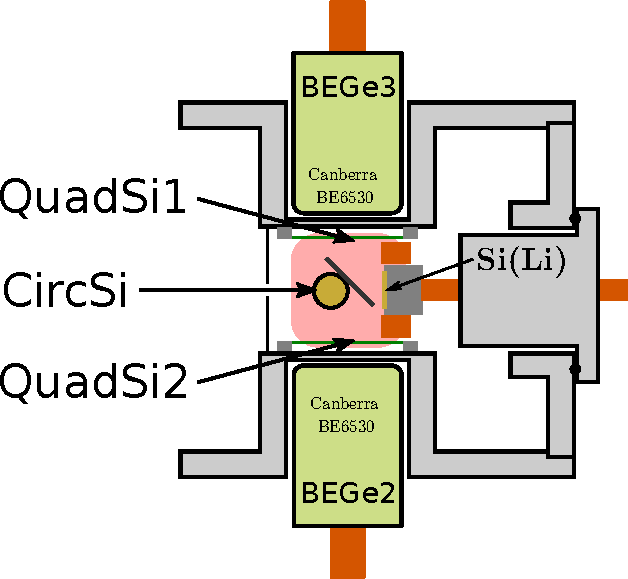
\includegraphics[width=1.\textwidth]{top_view.pdf}\\
	\end{column}
\end{columns}
\end{frame}

\begin{frame}{Sources}
	\begin{columns}
		\begin{column}{0.5\textwidth}
			\begin{overlayarea}{\textwidth}{\textheight}
				\centering
				\vspace{0.1\textheight}
				\begin{itemize}
					\item[1$\rightarrow$]<1->{3-$\alpha$ source \\
										\small$^{239}$Pu - $^{241}$Am - $^{244}$Cm}
					\item[5$\rightarrow$]<2->{$\gamma$ sources \\
										\small $^{133}$Ba - $^{210}$Pb - $^{60}$Co \\
										$^{137}$Cs - $^{152}$Eu}
					\item[1$\rightarrow$]<3->{$\alpha$-recoil source\\
										\small $^{223}$Ra}
				\end{itemize}
				\center
				\vspace{0.1\textheight}
				\hspace{-0.2\textwidth}
			\end{overlayarea}
		\end{column}
		\begin{column}{0.5\textwidth}
			\begin{overlayarea}{\textwidth}{\textheight}
				\centering
				\vspace{0.05\textheight}
				\only<1>{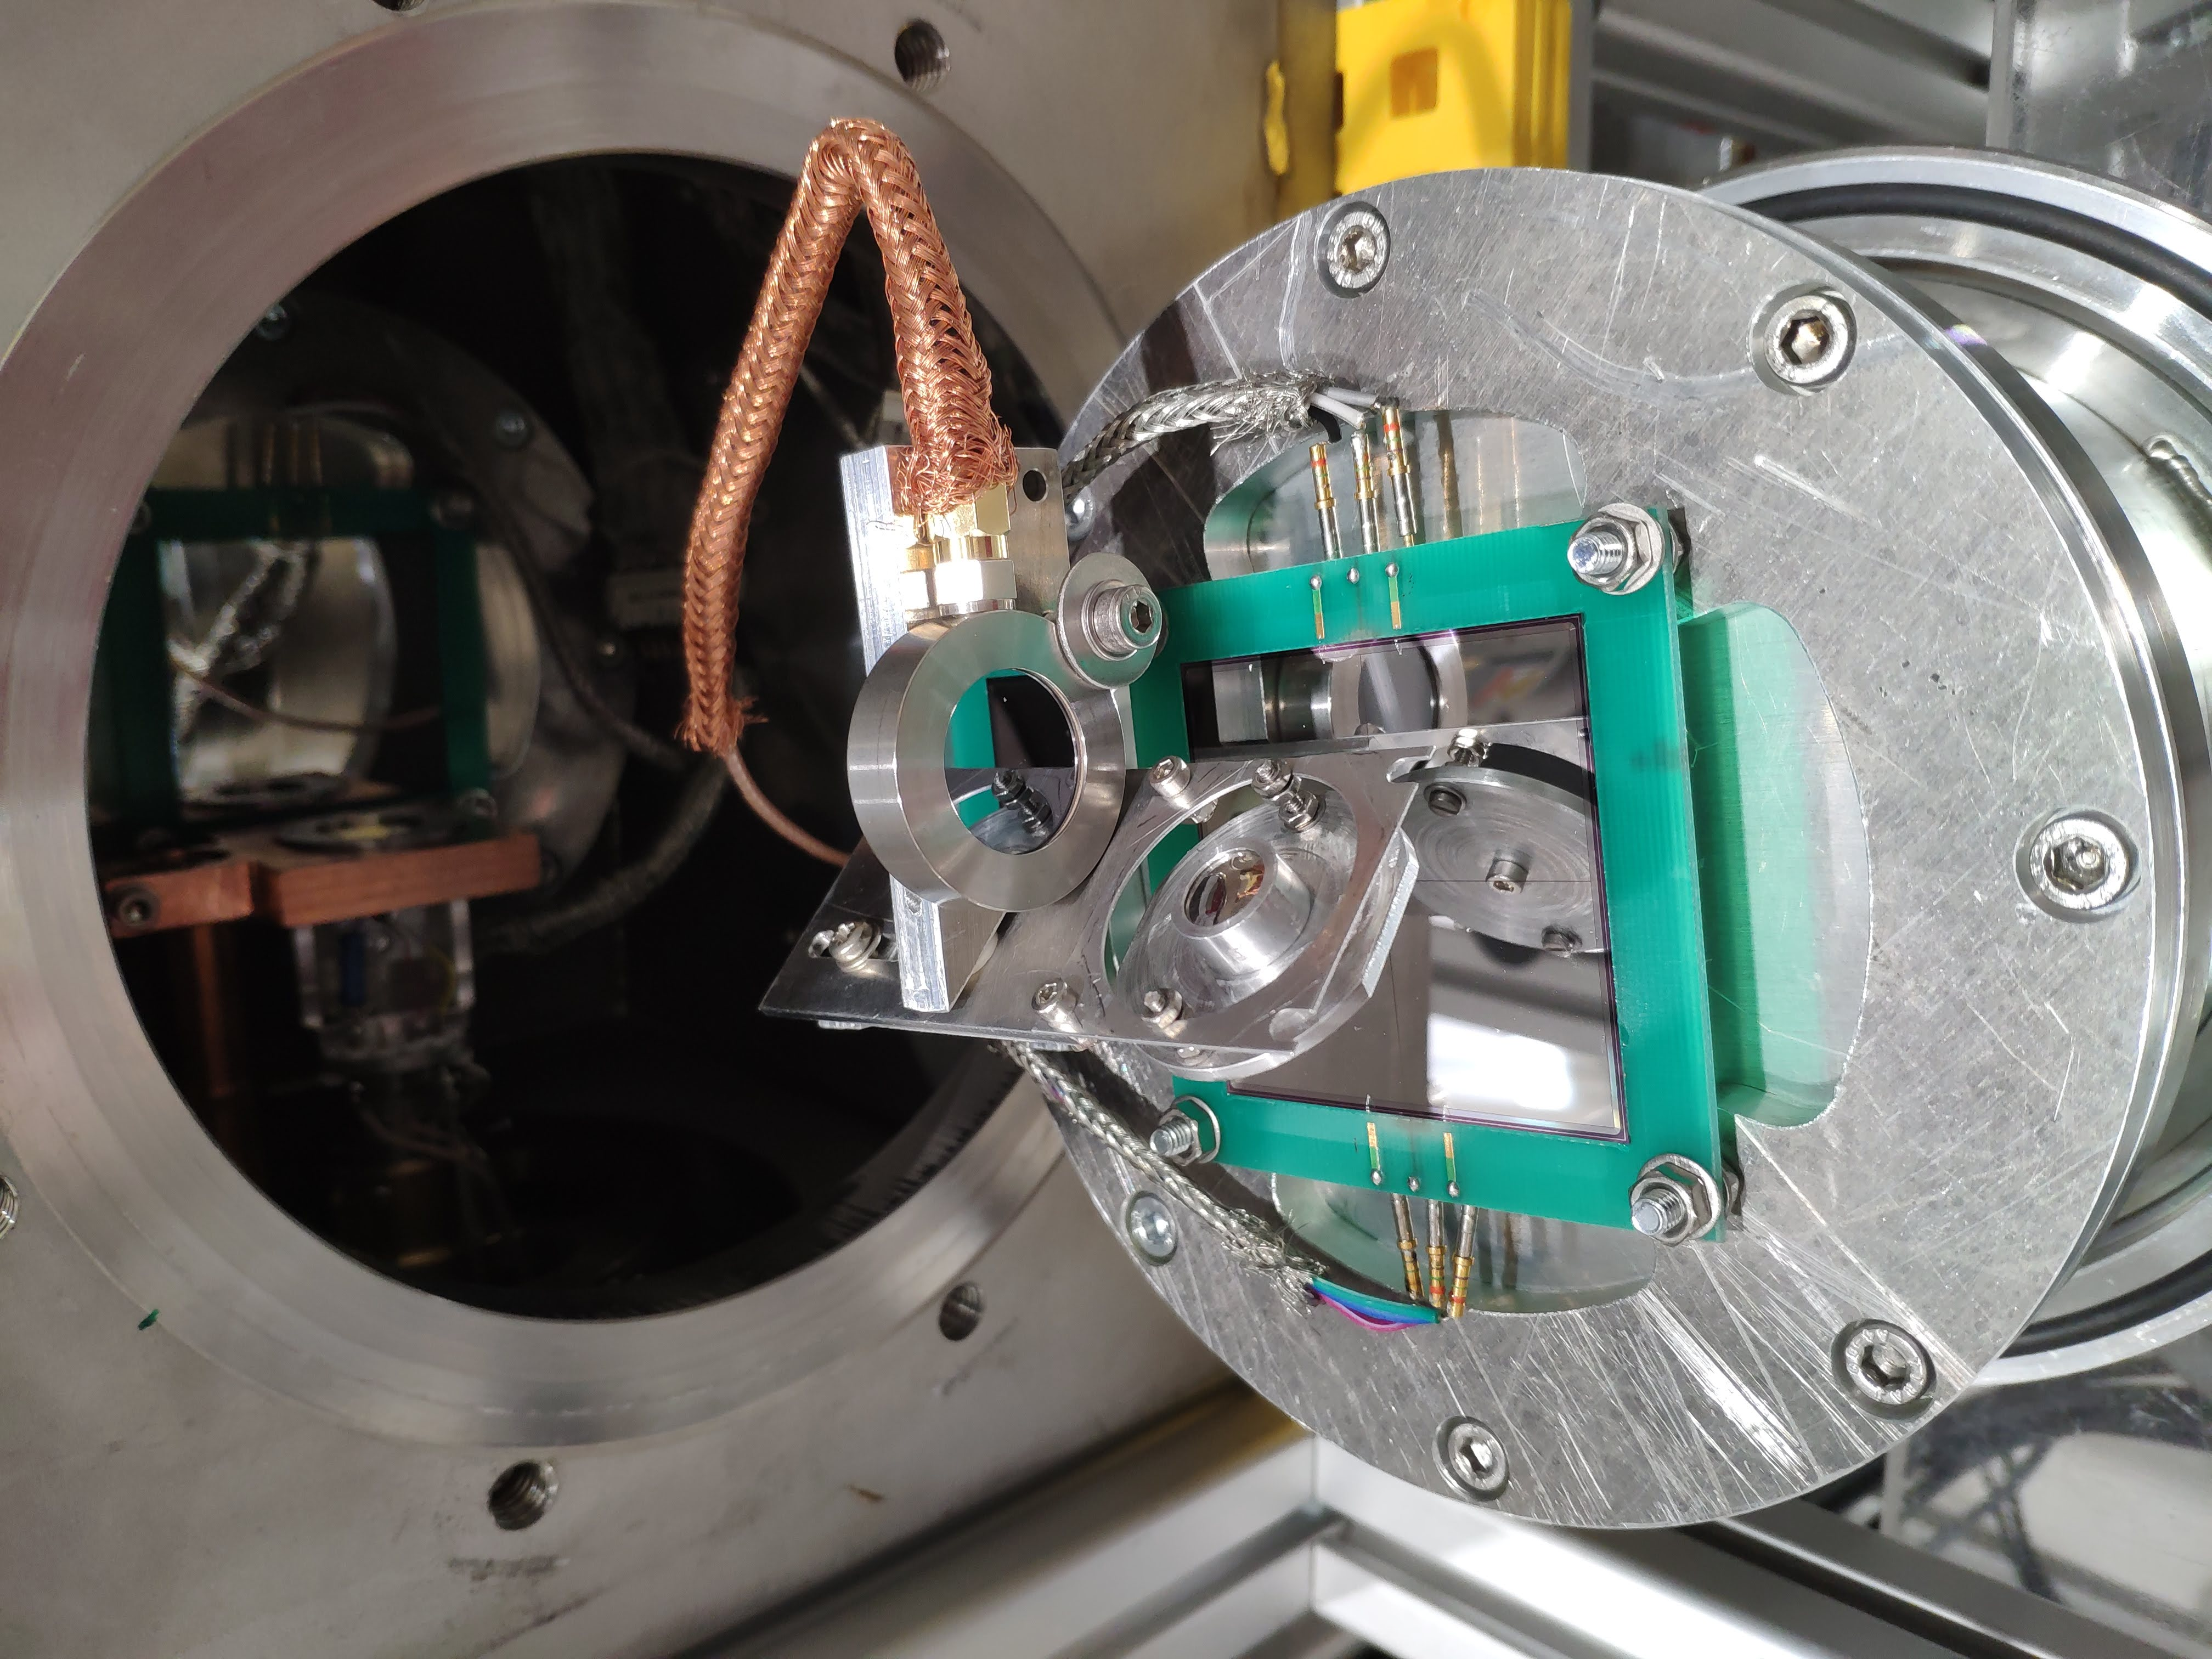
\includegraphics[angle=-90,origin=c,width=0.8\textwidth]{3alpha.jpg}}
				\only<2>{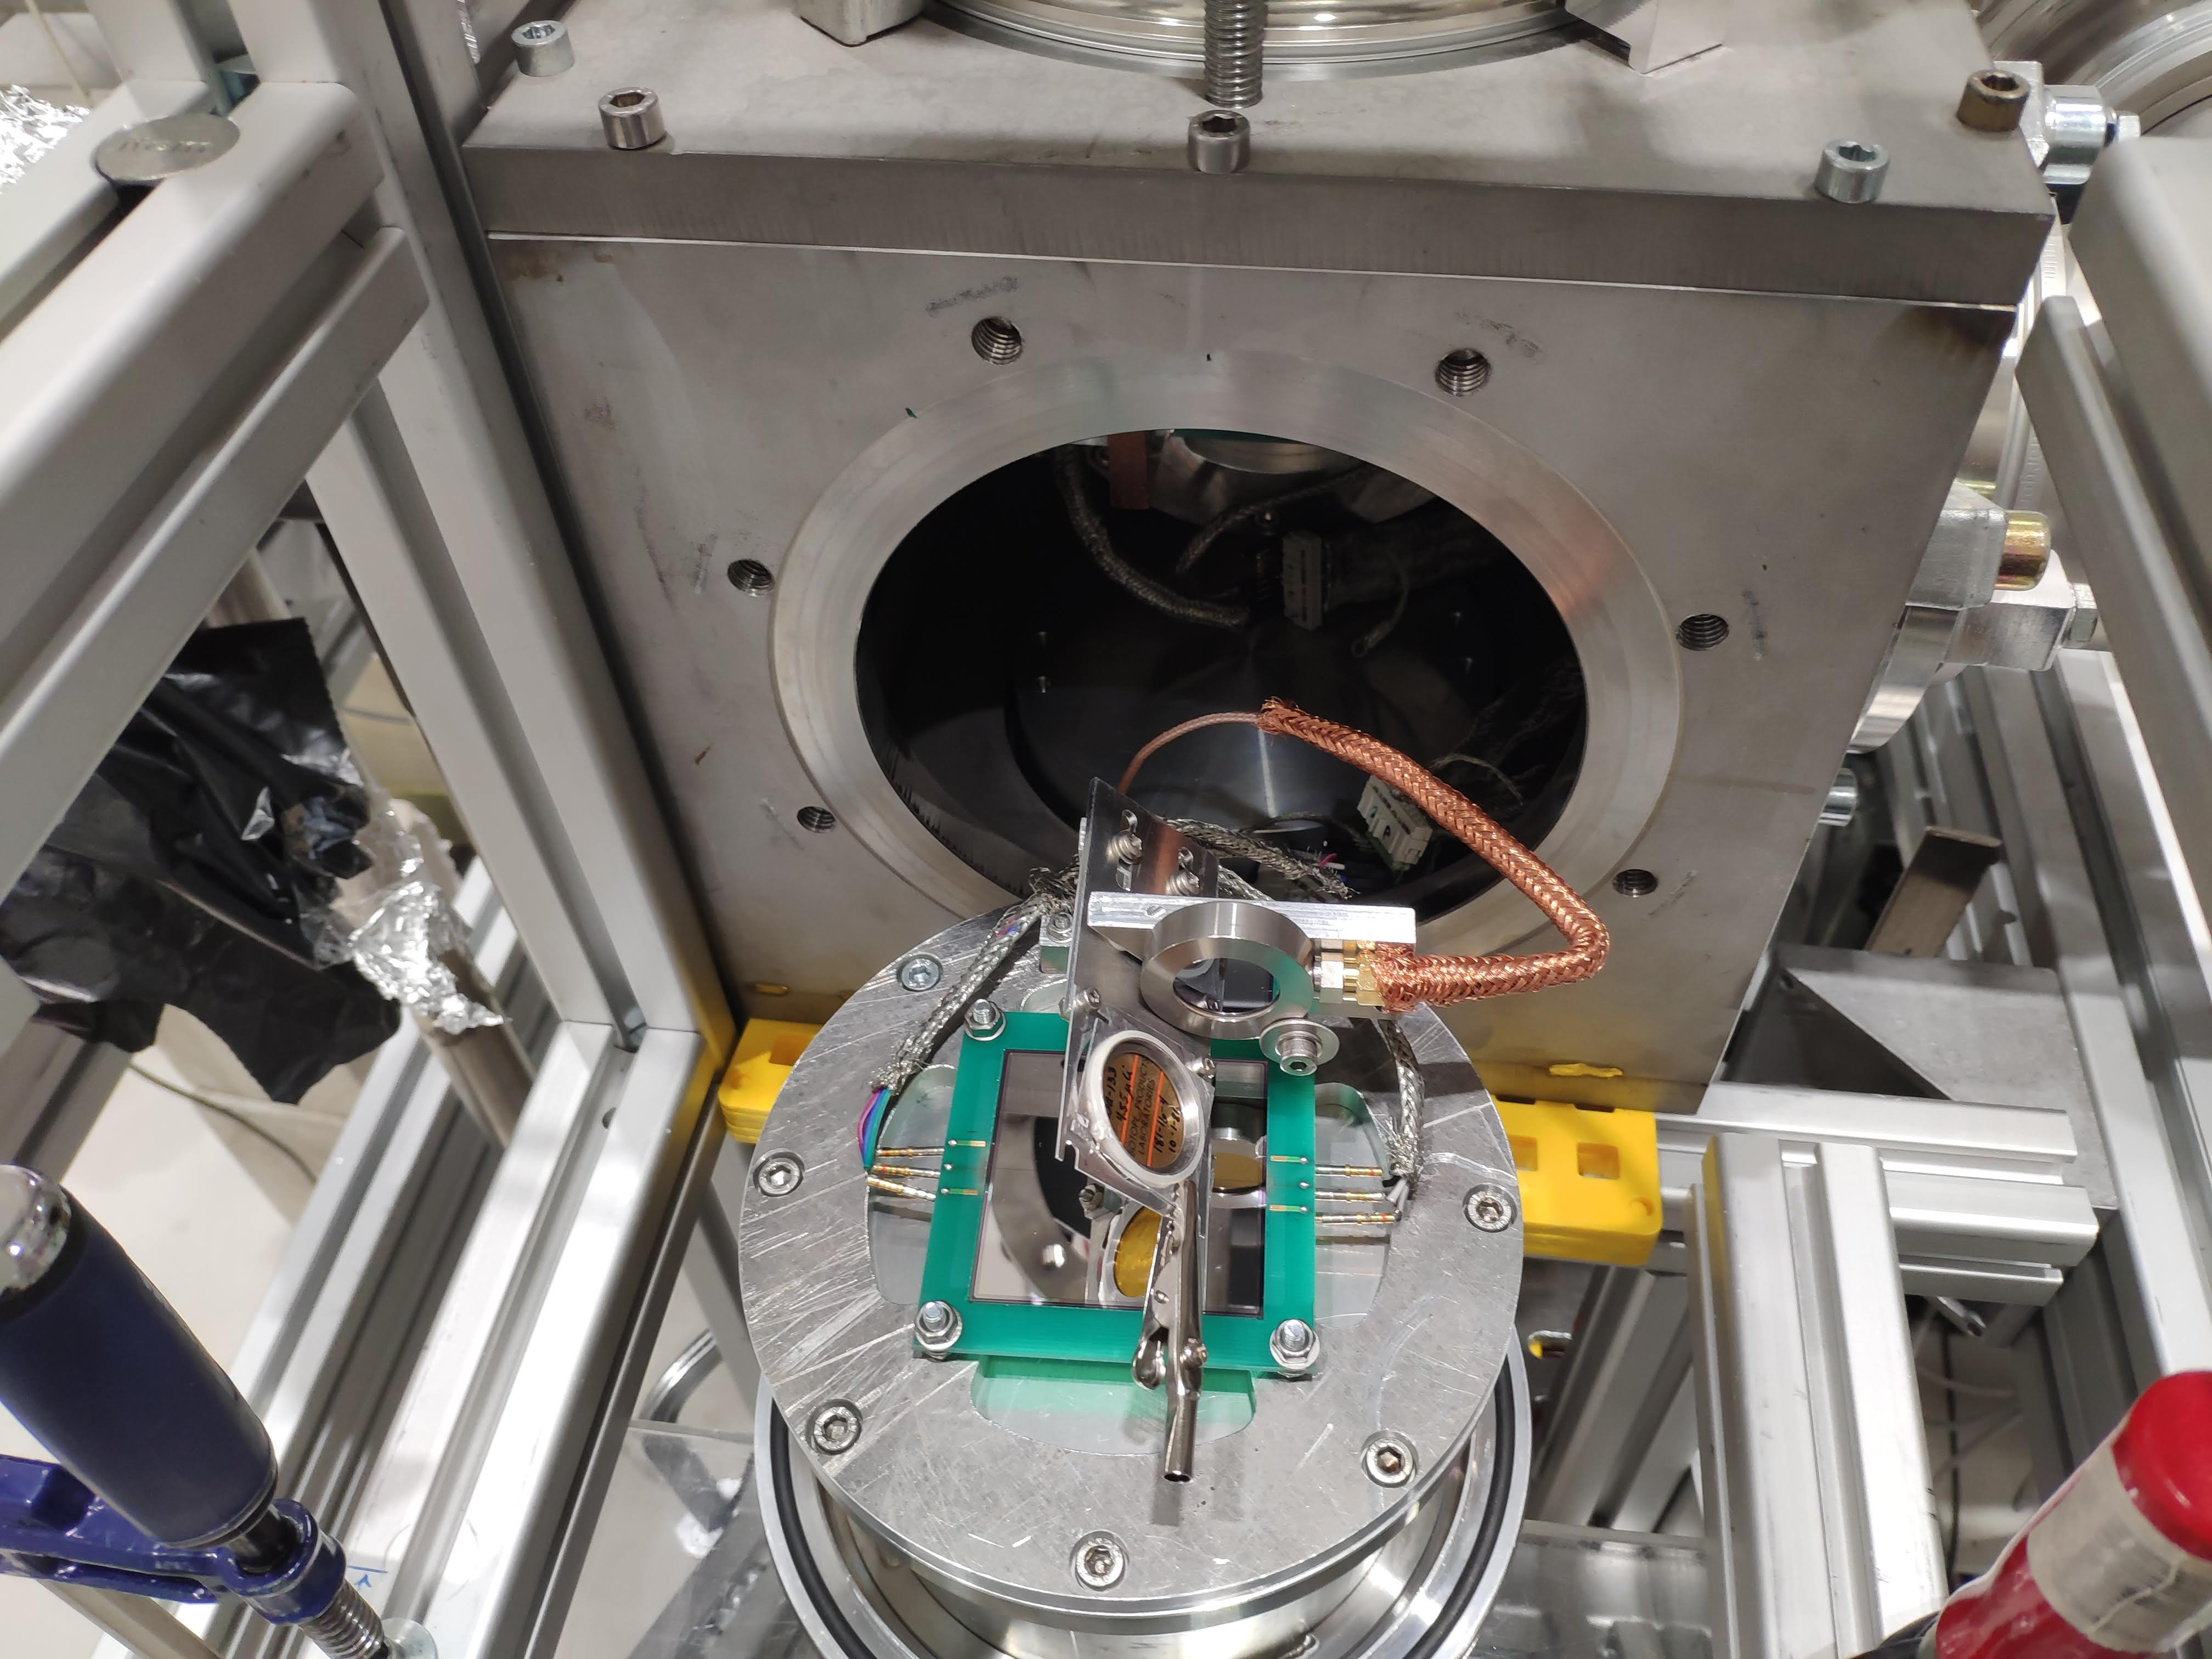
\includegraphics[width=1.\textwidth]{gammasrc.jpg}}
				\only<3>{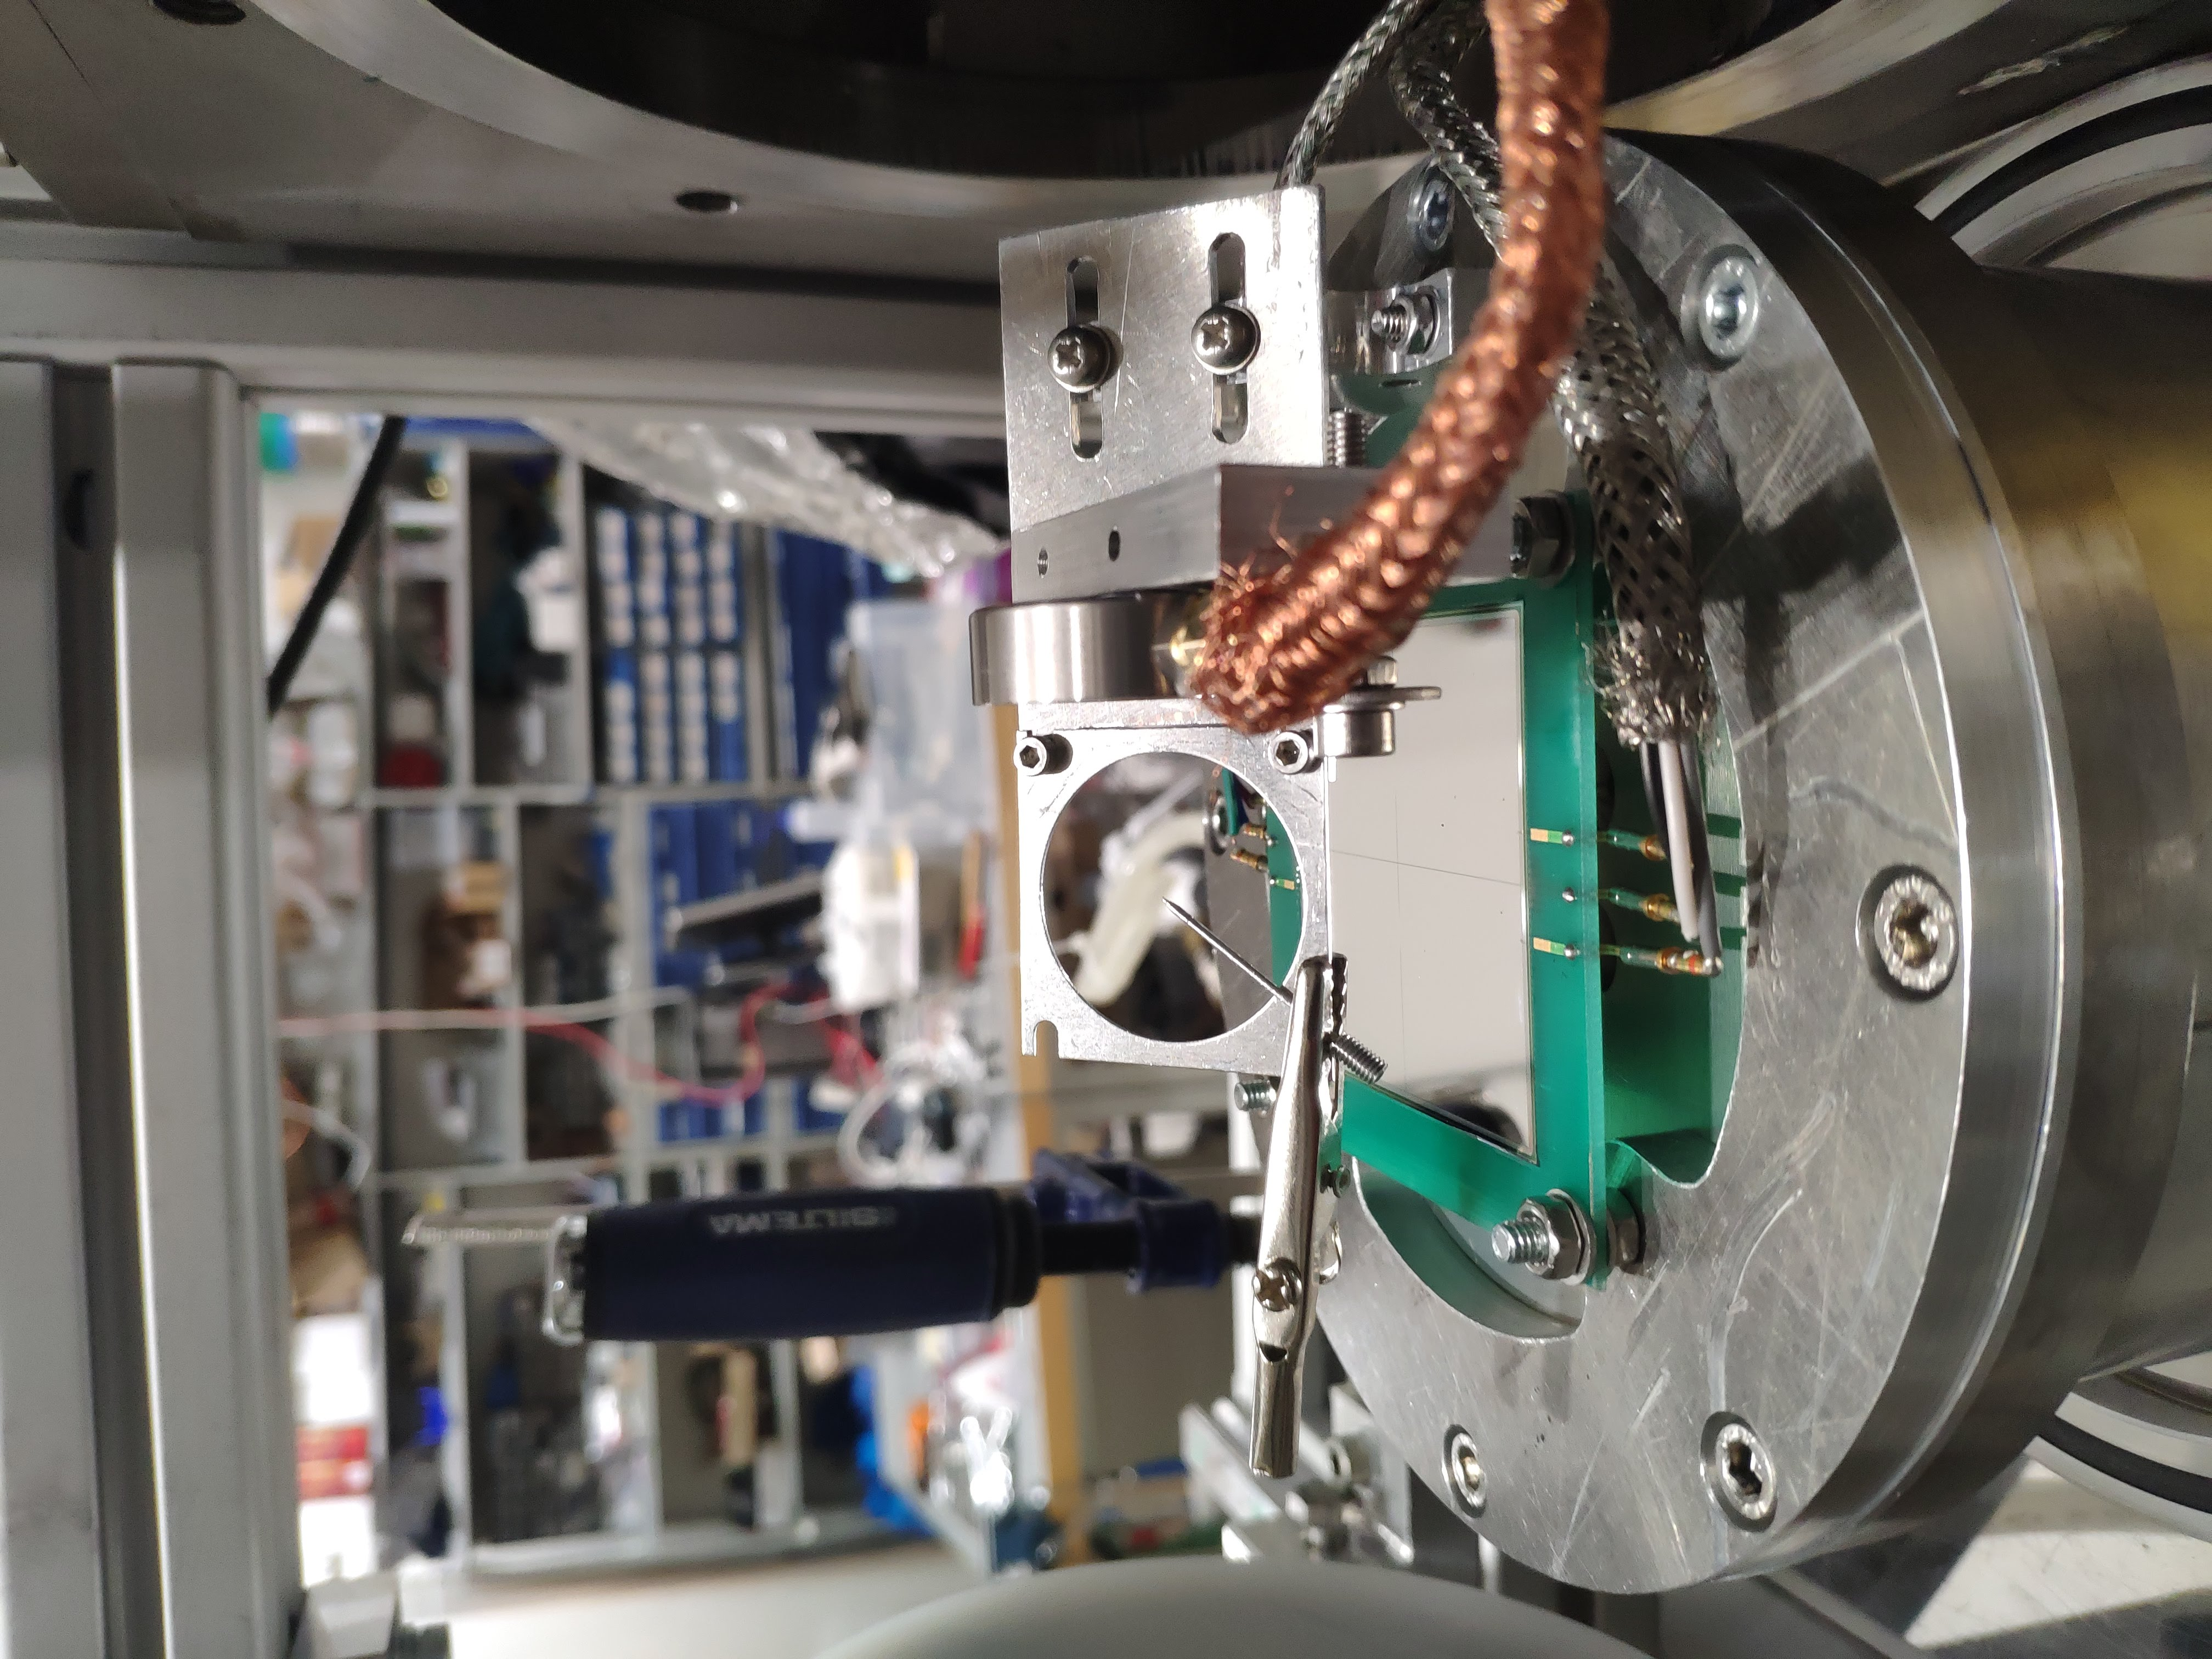
\includegraphics[angle=-90,origin=c,width=.8\textwidth]{alpharec.jpg}}
			\end{overlayarea}
		\end{column}
	\end{columns}
\end{frame}

\begin{frame}{BEGE Efficiency}
	\begin{columns}
		\begin{column}{0.4\textwidth}
			\begin{overlayarea}{\textwidth}{\textheight}
				\centering
				\small
				\[ \mathcal{E}_{\text{ABS}} = \dfrac{\text{Peak Area}}{\text{Time}\times \text{Activity}\times \text{Intensity}}\]
				\begin{itemize}
					\item[$\rightarrow$]<1-> Peak Area
					\item[$\rightarrow$]<2-> Time
					\item[$\rightarrow$]<3-> Activity
					\item[$\rightarrow$]<4-> Intensity
				\end{itemize}
			\end{overlayarea}
		\end{column}
		\begin{column}{0.6\textwidth}
			\begin{overlayarea}{\textwidth}{\textheight}
				\centering
				\vspace{0.15\textheight}
				\only<1>{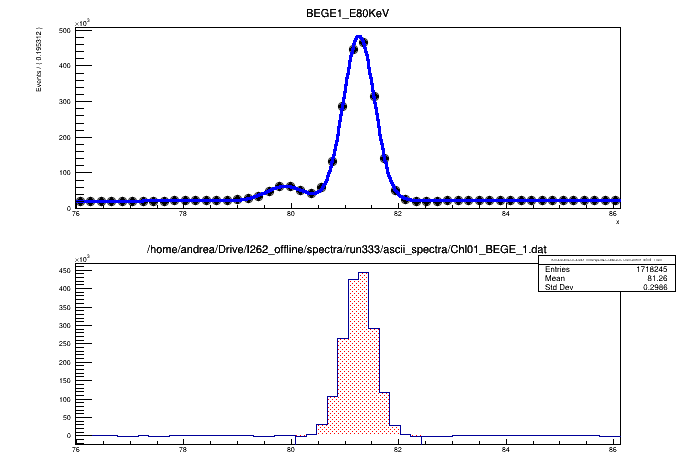
\includegraphics[width=\textwidth]{BEGE1_E80KeV.png}}
				\only<2>{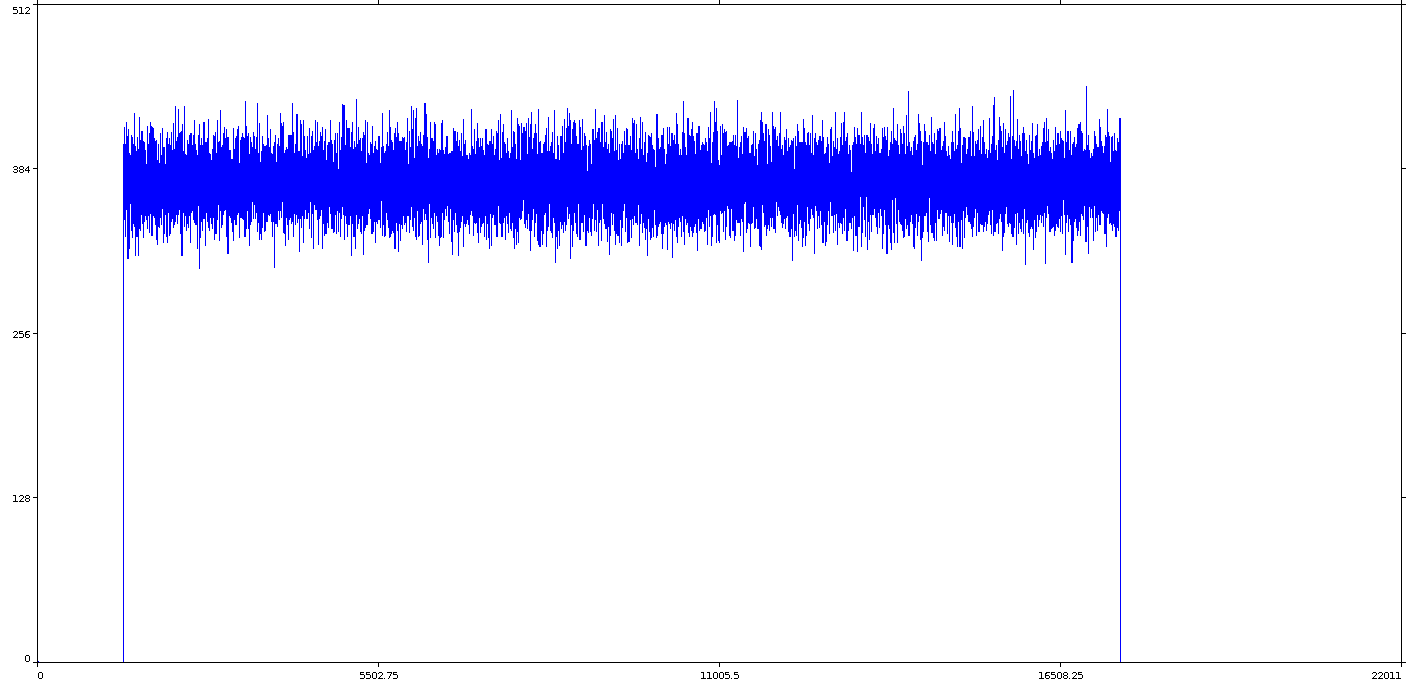
\includegraphics[width=\textwidth]{rates.png}}
				\only<3>{\[\text{A} = \text{A}_{0} \exp\left(-\ln\left(2\right)\dfrac{\Delta \text{T}}{\text{T}_{1/2}}\right)\]}
				\only<4>{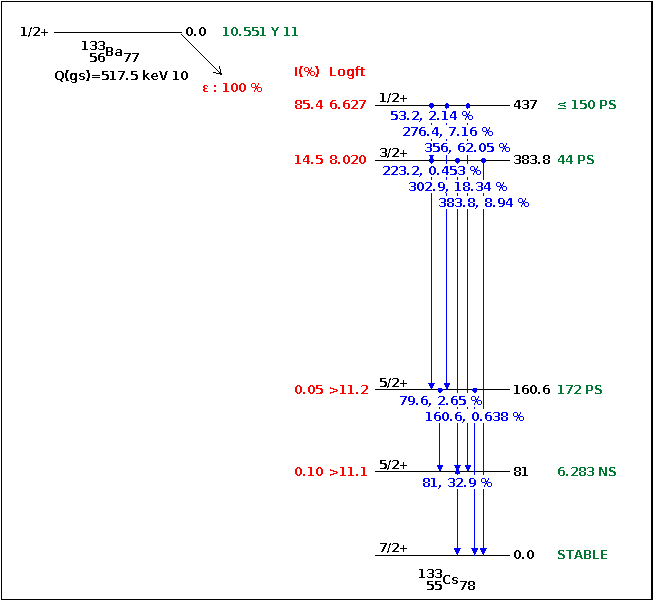
\includegraphics[width=.8\textwidth]{133Ba_decay.png}}
			\end{overlayarea}
		\end{column}
	\end{columns}
\end{frame}

\begin{frame}{BEGE Efficiency}
	\begin{columns}
		\begin{column}{0.5\textwidth}
			\begin{overlayarea}{\textwidth}{0.5\textheight}
				\centering
				\textbf{Vertical Axis}
				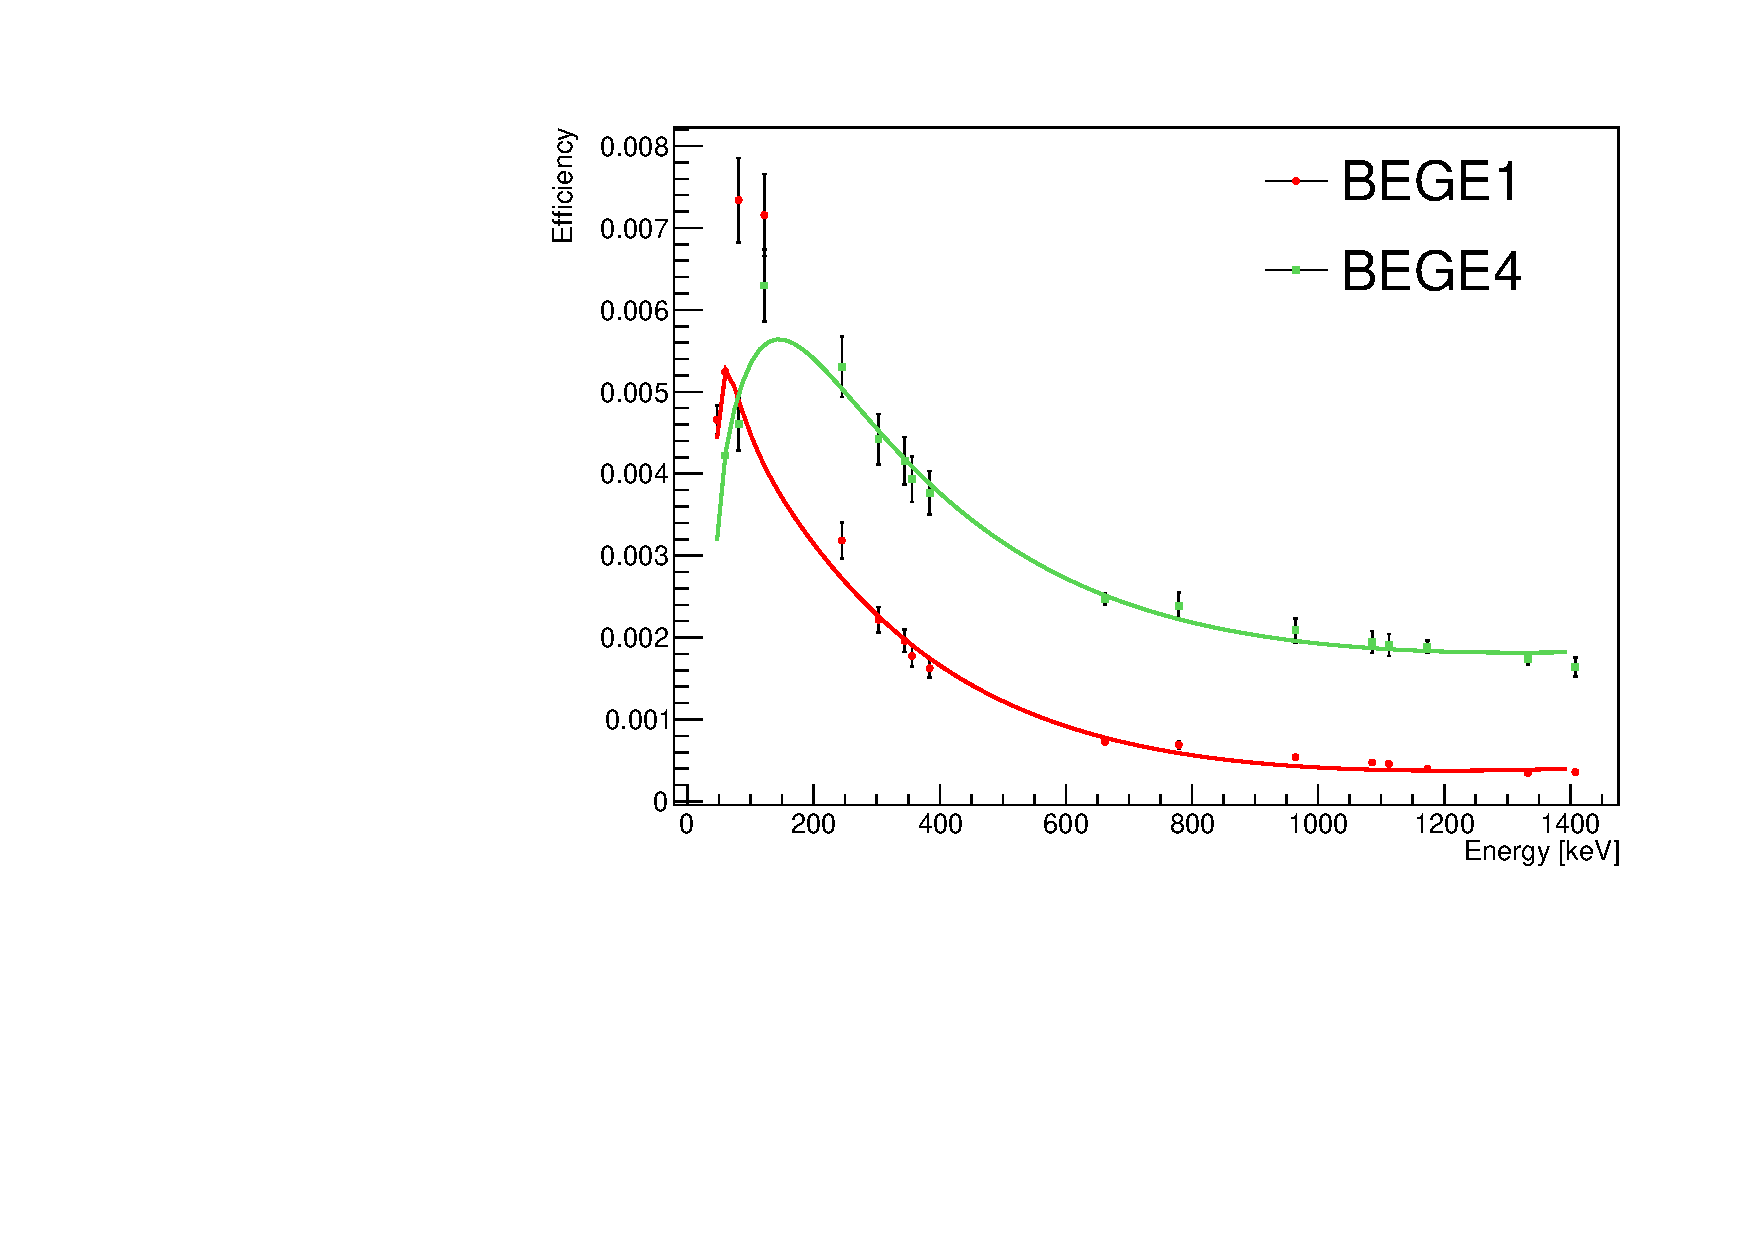
\includegraphics[width=\textwidth]{GraysBEGE1-4.pdf}
			\end{overlayarea}
		\end{column}
		\begin{column}{0.5\textwidth}
			\begin{overlayarea}{\textwidth}{0.5\textheight}
				\centering
				\textbf{Horizontal Axis}
				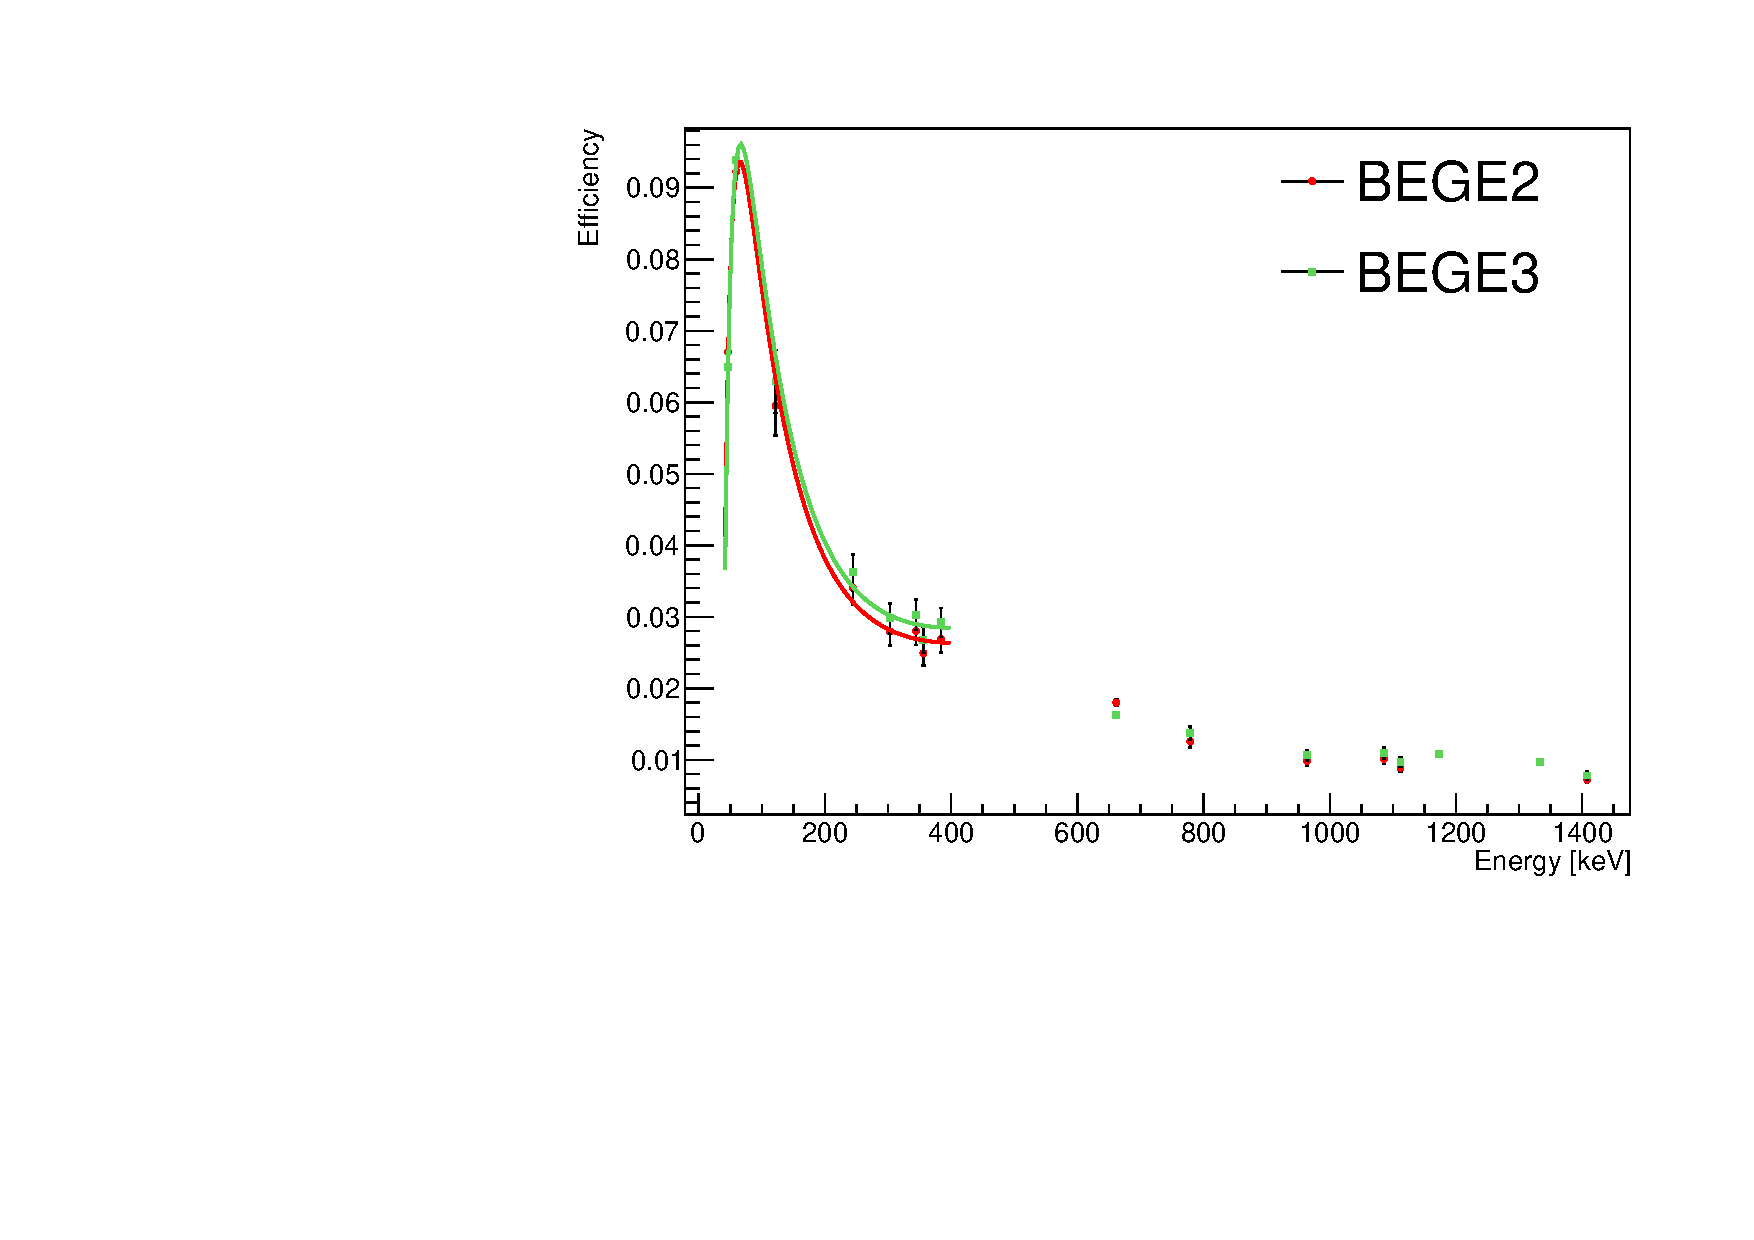
\includegraphics[width=\textwidth]{GraysBEGE2-3_fullrange.pdf}
			\end{overlayarea}
		\end{column}
	\end{columns}
	\small
	$\footnote{\tiny Hurtado Garcia-Lenon Nucl. Instr. and Meth. A 594 (2008) 362–367} \mathcal{E}_{\text{ABS}} (E) = a_1 \left(\exp \left(-a_2 E^{a_3}\right)+\exp \left(-a_4 E^{a_5}\right)	\right)\left(1-\exp \left(a_6 E^{a_7}\right)\right) $\\
	$\footnote{\tiny P.W. Gray, A. Ahmad, Nucl. Instr. and Meth. A 237 (1985) 577}\color{red} \mathcal{E}_{\text{ABS}} (E) = \dfrac{1}{E}\sum_i a_i \left(\ln(E)\right)^{i-1}$
\end{frame}

\begin{frame}{Error sources}
	\begin{columns}
		\begin{column}{0.5\textwidth}
			\begin{overlayarea}{\textwidth}{\textheight}
				\centering
				\small
				\begin{itemize}
					\item[$\rightarrow$]<1-> Integral error \color{green}\checkmark
					\item[$\rightarrow$]<2-> acquisition time error\\ (negligible ?)
					\item[$\rightarrow$]<3-> {Half Life time error\\ (negligible ?)}
					\item[$\rightarrow$]<4-> Original Activity Error \color{green}\checkmark
					\item[$\rightarrow$]<5->{Intensity \\
											\begin{itemize}
												\item Intensity error \text{\color{green} \checkmark}
												\item Coincidence summing $\gamma$
											\end{itemize}}
					\item[$\rightarrow$]<6->{Geometrical error\\
											\begin{itemize}
												\item Isotropic emission
												\item Point-like source
											\end{itemize}} 
				\end{itemize}
			\end{overlayarea}
		\end{column}
		\begin{column}{0.5\textwidth}
			\begin{overlayarea}{\textwidth}{\textheight}
				\centering
				\only<5>{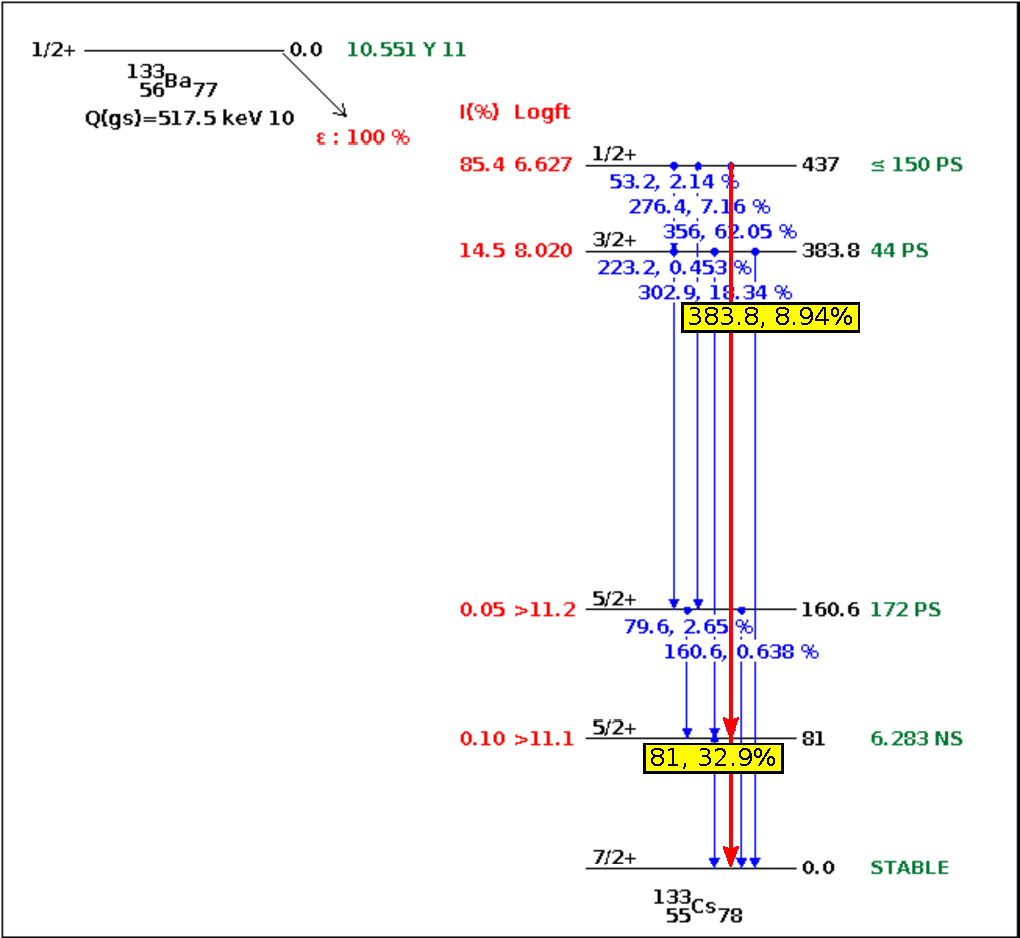
\includegraphics[width=\textwidth]{133Ba_summing.pdf}}
				\only<6>{\vspace{0.1\textheight}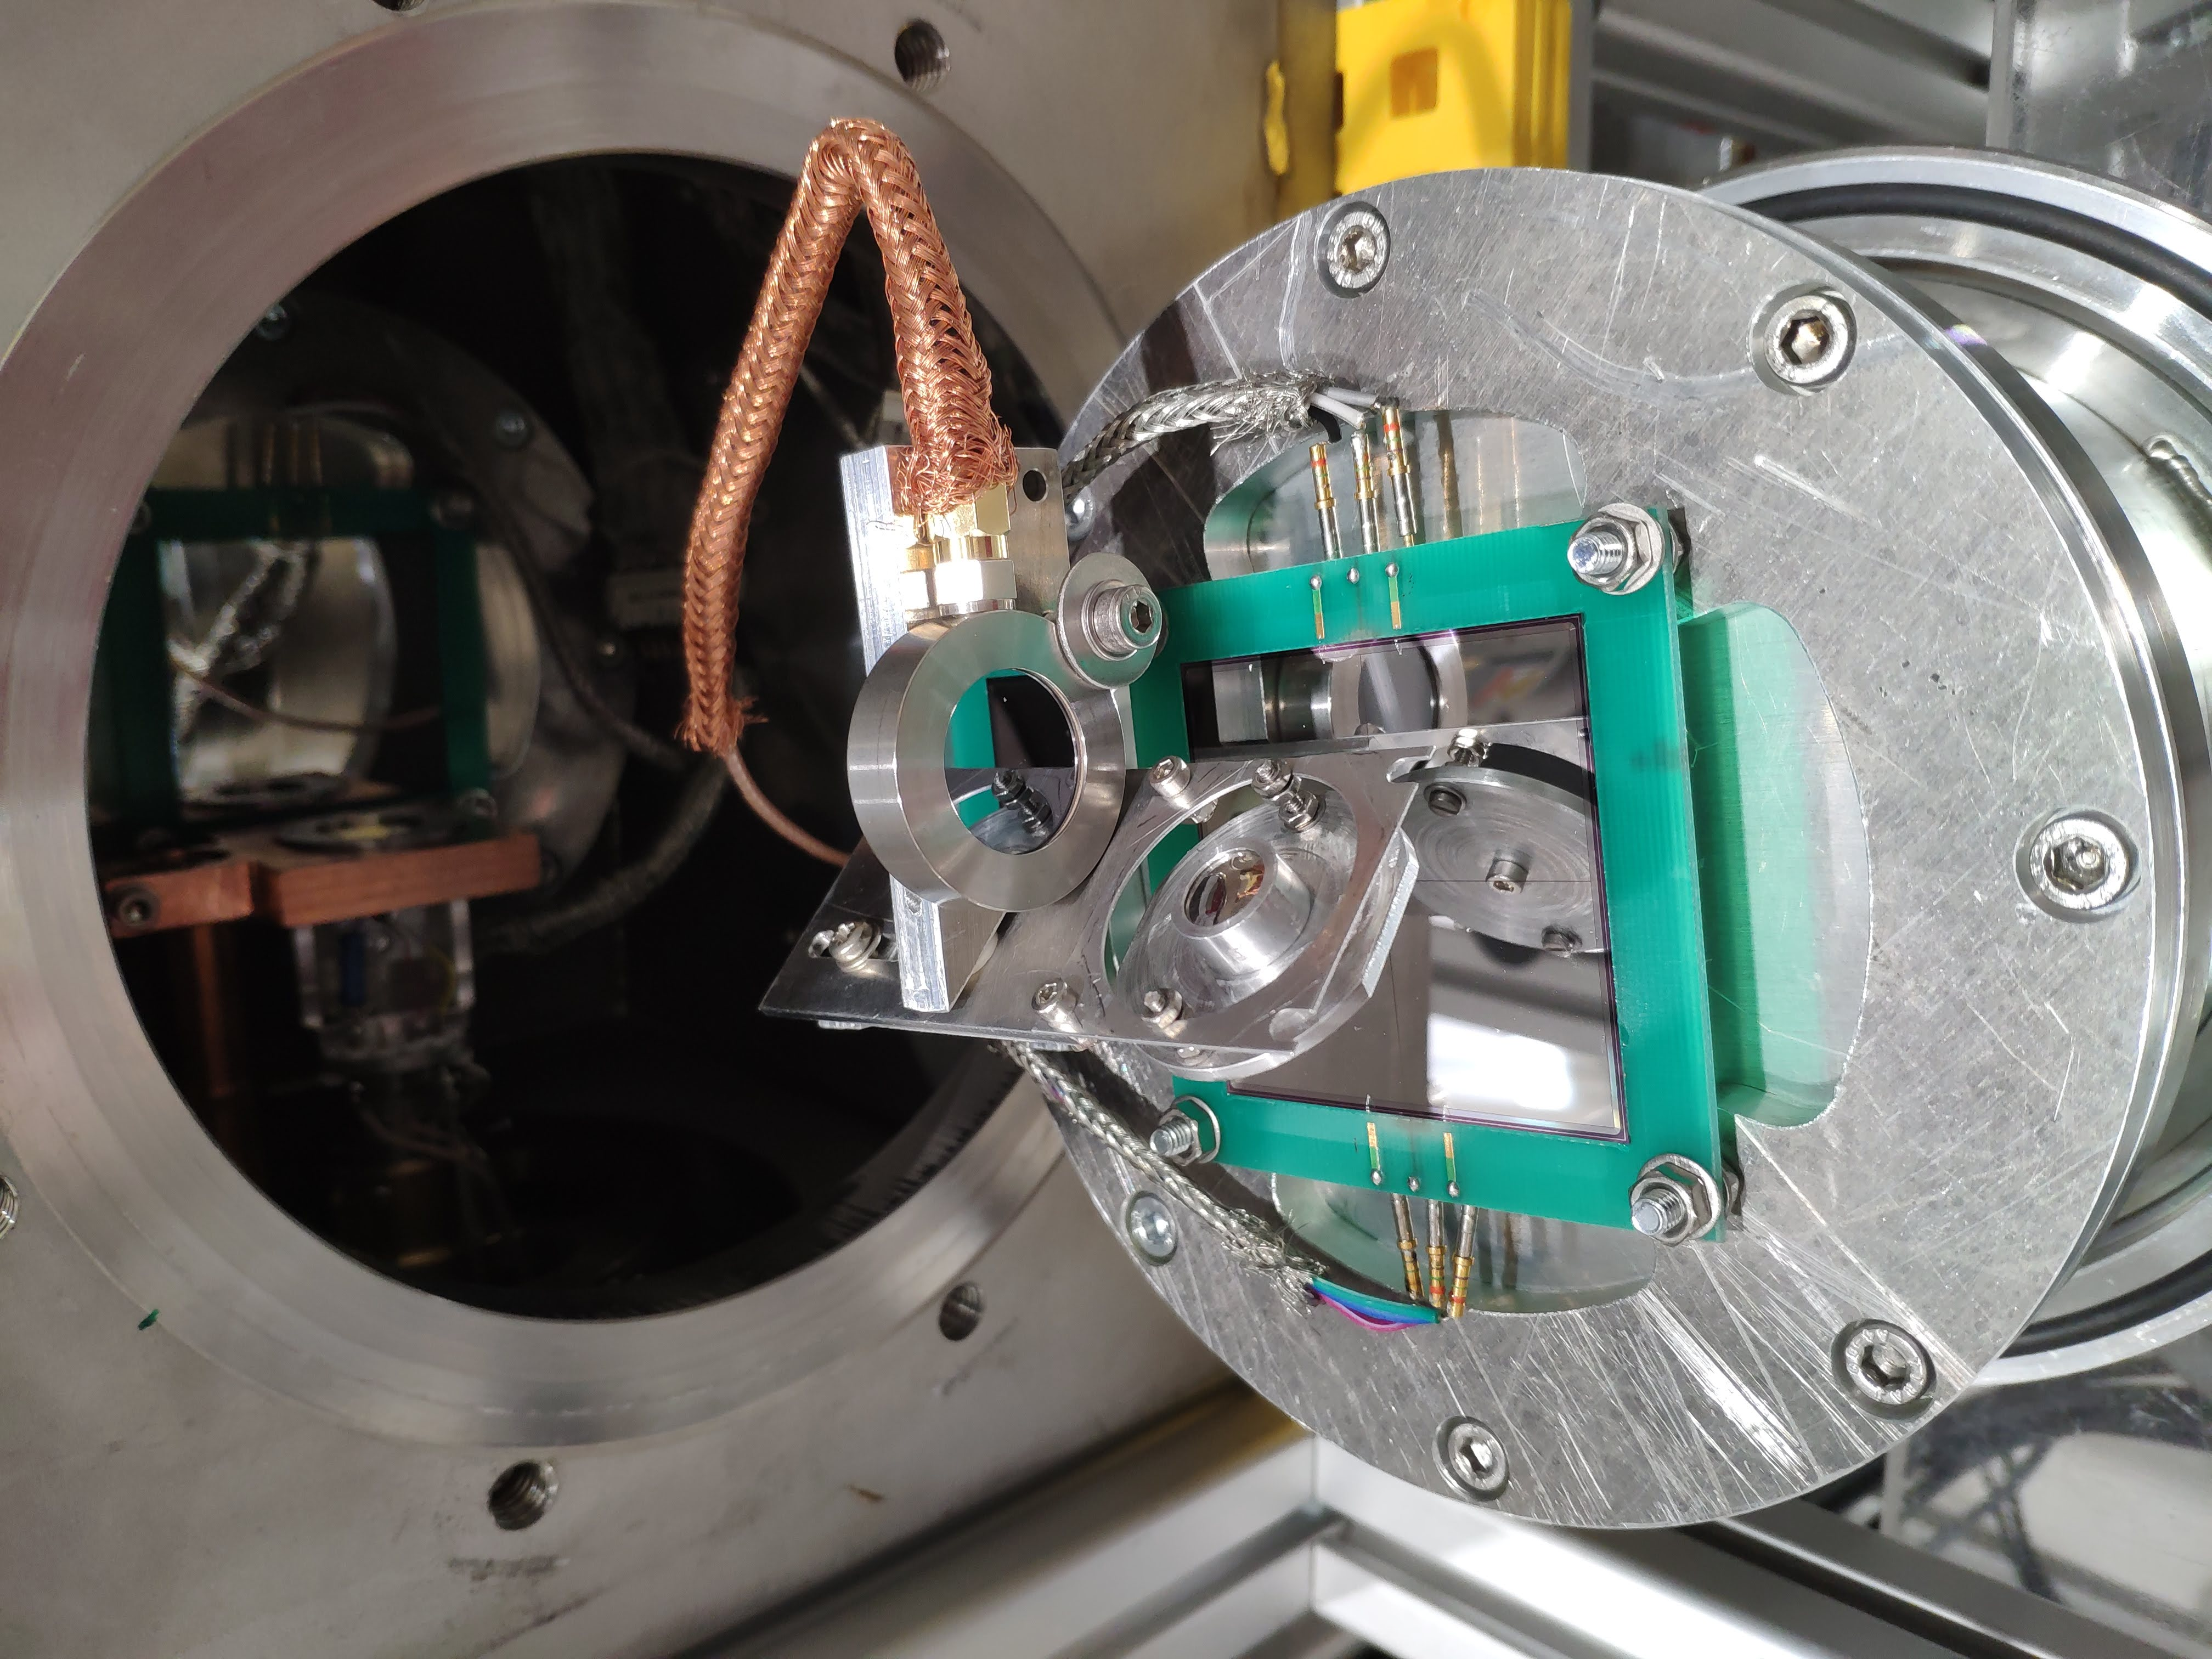
\includegraphics[angle=-90,origin=c,width=0.45\textwidth]{3alpha.jpg}
				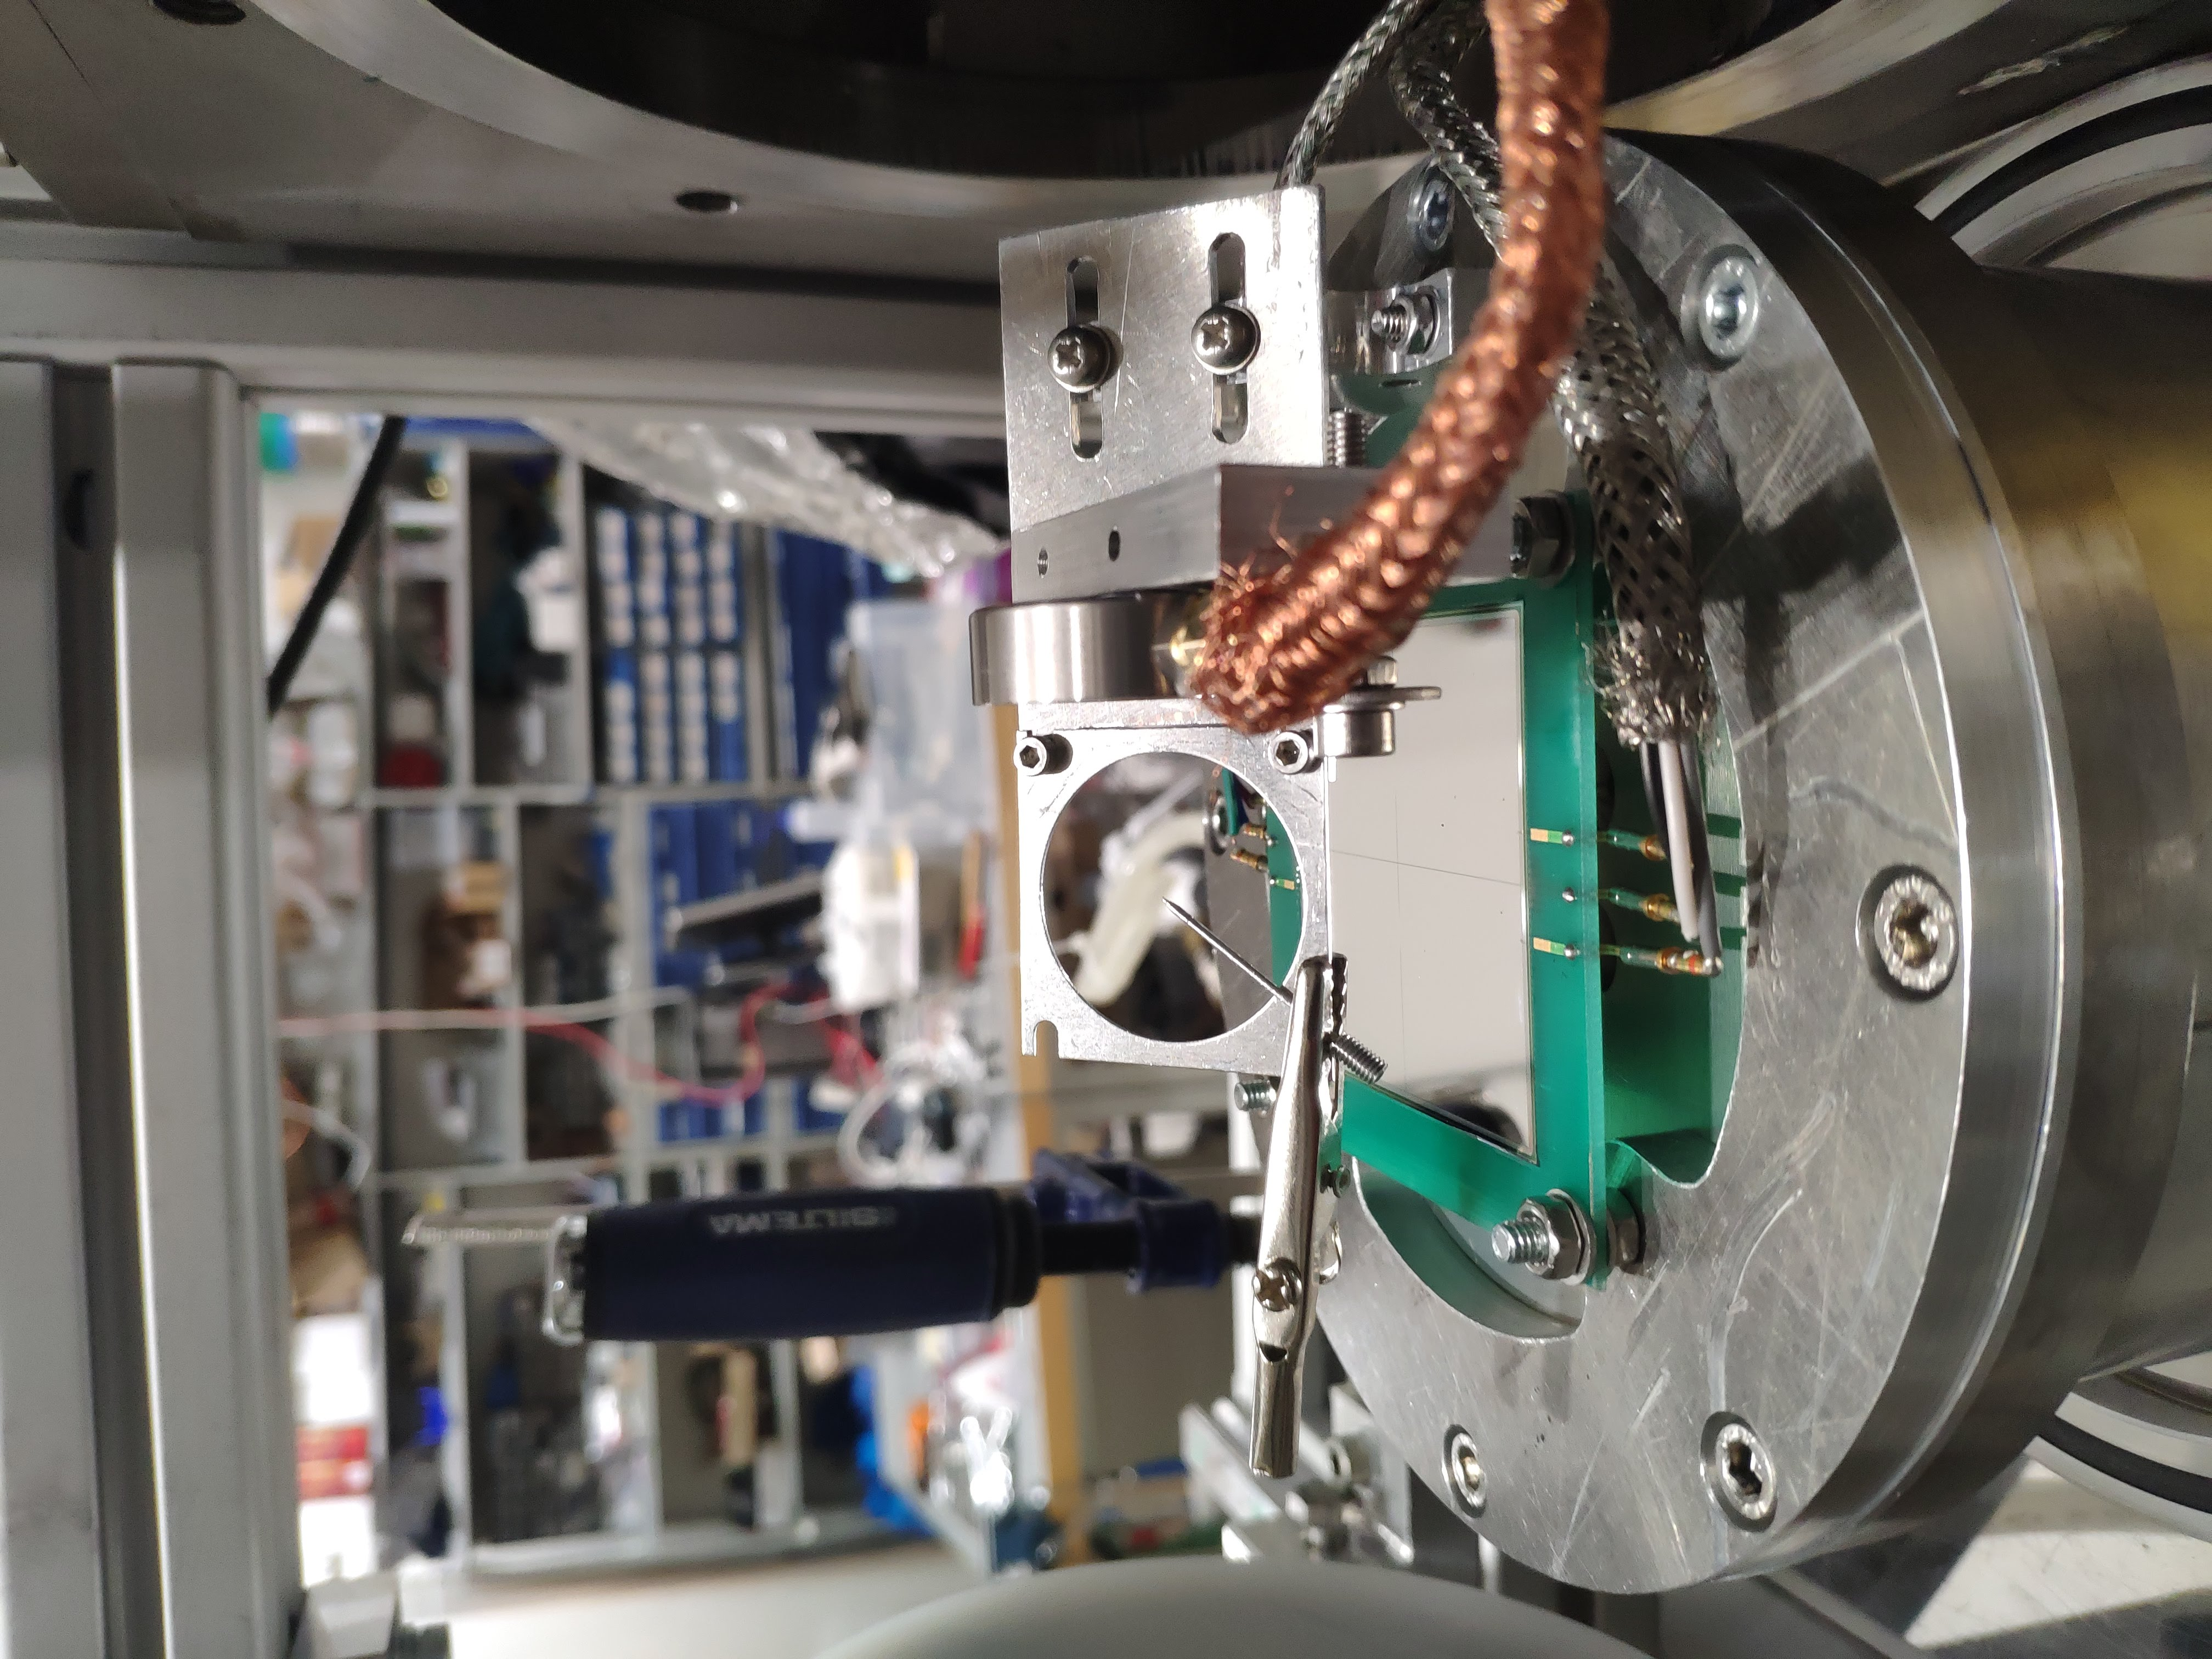
\includegraphics[angle=-90,origin=c,width=0.45\textwidth]{alpharec.jpg}}
			\end{overlayarea}
		\end{column}
	\end{columns}
\end{frame}

\begin{frame}{223Ra $\alpha$-recoil source}
	\centering
	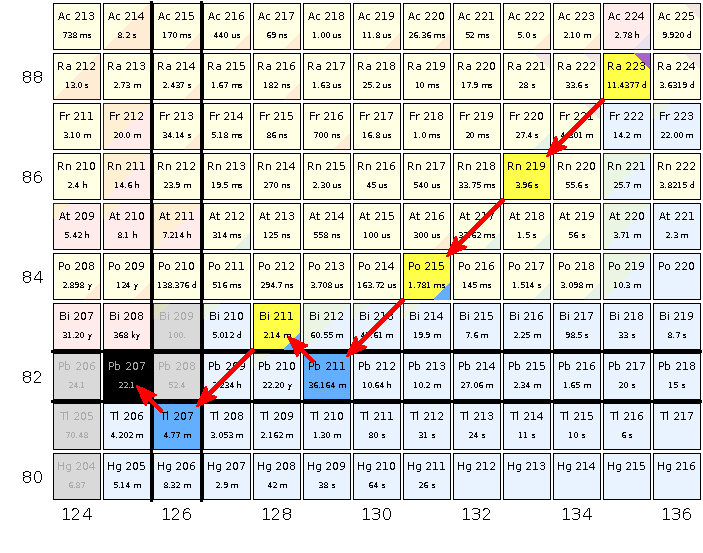
\includegraphics[width=.8\textwidth]{chart.pdf}
\end{frame}

\begin{frame}{223Ra $\alpha$-recoil source}
	\centering
	\vspace{-0.1\textheight}
	\textbf{Activity measurment before and after the acquistion with the setup}\\
	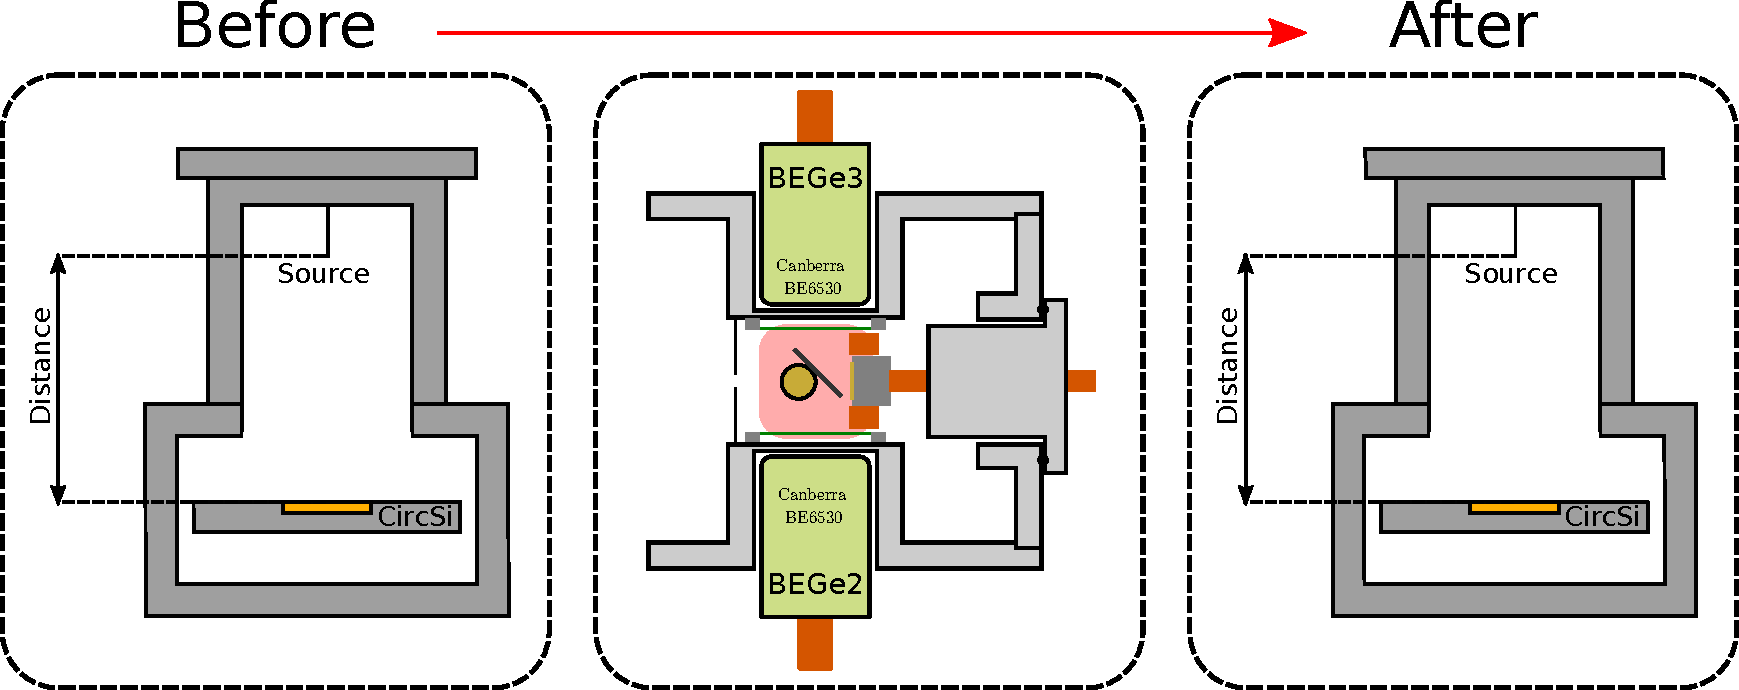
\includegraphics[width=.9\textwidth]{activity_setup.pdf}
\end{frame}


\begin{frame}{223Ra $\alpha$-recoil source}
	\centering
	\vspace{-0.1\textheight}
	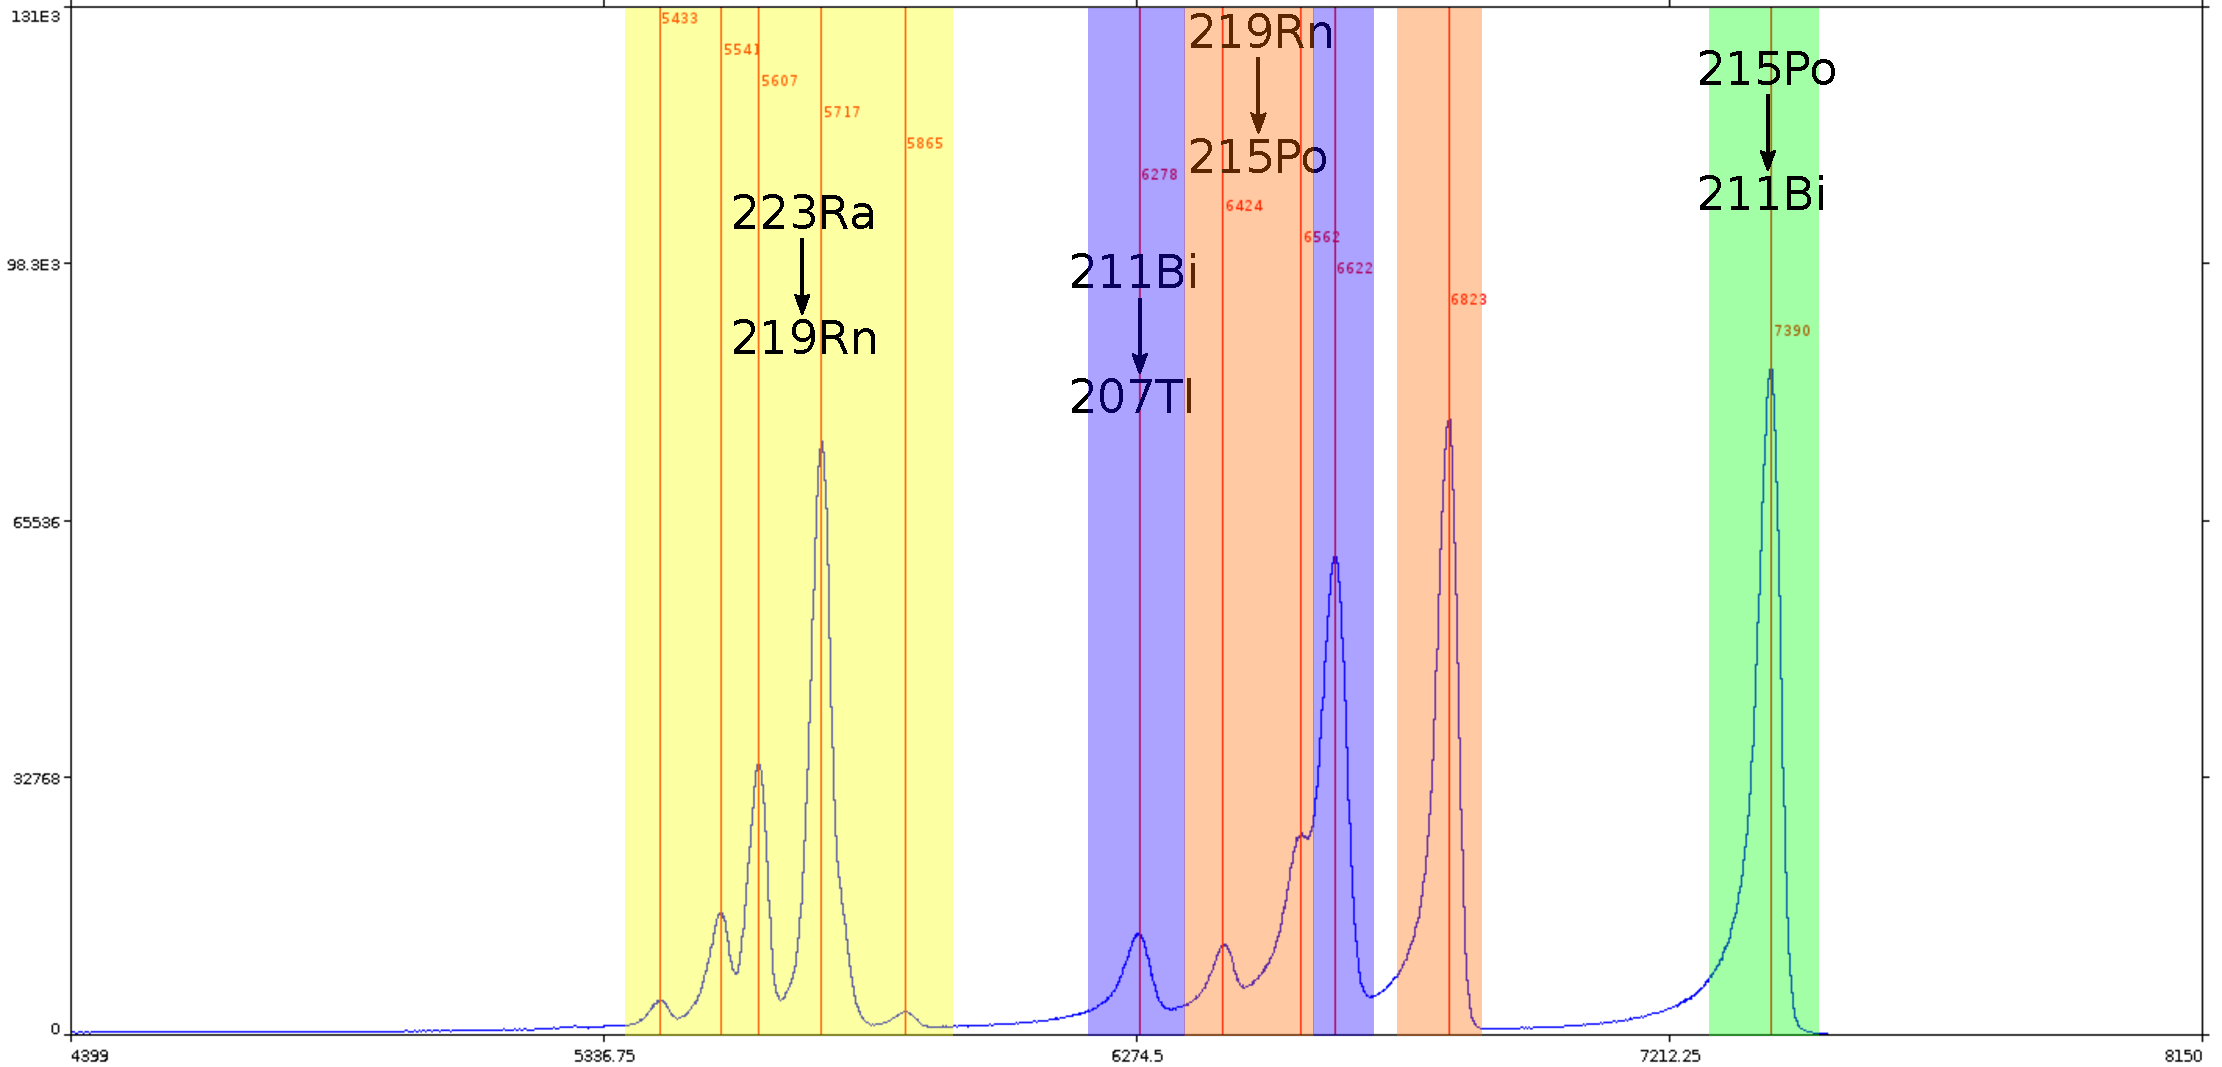
\includegraphics[width=.9\textwidth]{alpharec_spectra.pdf}
\end{frame}


\begin{frame}{To Do List}
	\centering
	\begin{itemize}
		\item Efficiency curves fitting
		\item Include 3-$\alpha$ source $^{241}$Am low energy $\gamma$ 
		\item Include correction coefficients for coincident summing
		\item Compute geometrical error contribution
		\item Compute Si detectors efficiency from $^{223}$Ra source spectra.
	\end{itemize}
\end{frame}

\end{document}